 %!TEX root = ../thesis.tex
%*******************************************************************************
%****************************** Second Chapter *********************************
%*******************************************************************************
\part{État de l'art}
\chapter{Les EIAH pour l'apprentissage de gestes}
Ce chapitre présente un état de l'art sur les différents éléments nécessaires à la conception d'EIAH pour soutenir l'apprentissage humain de gestes. La première partie rappelle et décrit l'une des représentations informatiques les plus connues pour modéliser le mouvement humain i.e. la représentation par une succession temporelle de squelettes. La seconde partie fait état des différents moyens pour capturer le mouvement. La troisième partie se concentre sur les EIAH existants, le matériel utilisé pour la capture, leurs principales caractéristiques (\textit{e.g.} domaines applicatifs, types de données utilisées, etc.) et les retours faits à l'apprenant. De plus, elle étudie ces systèmes sous l'angle de la réingénierie et la place/le rôle des usagers au sein de ces systèmes.

%REFAIRE L'INTRO (obviously)

Dans la suite de ce manuscrit, nous utiliserons le terme de « geste cible », pour faire référence au geste à apprendre pour atteindre l'objectif de la tâche à réaliser. En effet, il existe parfois, pour une même tâche d'apprentissage, plusieurs gestes possibles jugés corrects par un ou plusieurs experts. Ces gestes constituent l’objectif d’apprentissage. Si l'on prend l'exemple du service au tennis, et que l'on définit la tâche comme étant le fait de frapper la balle de manière à ce qu'elle arrive dans la zone légale de service adverse, plusieurs mouvements existent : le lancer " droit ", le lancer " arrière " et le lancer " devant ". De plus, il est possible d'imprimer un effet à la balle lors de la frappe (\textit{lifté} ou \textit{slicé}), ce qui induit une variation du geste de frappe \parencite{Zappala2017IoP}. Au bowling, il existe à minima trois types de lancers différents (\textit{Stroker}, \textit{Cranker}, \textit{Spinner}) pour atteindre l'objectif, qui est de renverser un maximum de quilles en un minimum de lancers  \parencite{Tan2000Cbp}. Ces deux exemples parmi tant d'autres montrent qu'il ne serait possible de définir un seul geste comme étant le geste parfait à atteindre pour une situation d'apprentissage donnée. En conséquence, nous introduisons le terme de " geste cible ", qui est le geste dont les caractéristiques sont : (i) connues par l'expert et (ii) doivent être transmises à, et maîtrisées par, l'apprenant. Le geste cible peut être différent d'un expert à l'autre pour un mouvement donné, en fonction de l'objectif recherché et des spécificités morphologiques.

%DANSE : \parencite{Maes2012DtM} (a mettre dans le tableau)

\section{Représentation du mouvement}
Afin de pouvoir exploiter les données de mouvement au sein d'un EIAH, il faut pouvoir formaliser, discrétiser puis opérationnaliser les mouvements du corps. Une des techniques les plus utilisées consiste à utiliser des graphes, et plus particulièrement des arbres, afin de modéliser les mouvements du corps humain sous la forme d'une succession de squelettes 3D, c'est-à-dire des postures espacées selon un pas de temps fixe ou variable \parencite{Lewis2000Psd}.

Le corps humain peut ainsi être vu comme un ensemble structuré d'articulations sous la forme d'une arborescence (Fig. \ref{fig:3D_skeleton_tree_example}). Dans ce cas, les nœuds de l'arbre représentent les articulations, et les arcs représentent les différents membres du corps.

\begin{figure}[h]
    \centering
    \includegraphics[width=5cm]{pictures/3D_skeleton_tree_example.png}
    \caption[Représentation informatique d'un squelette humain en 3D]{Un exemple de squelette humain 3D représenté sous la forme d'un arbre. Les articulations sont représentées à l'aide de nœuds (en vert), et les membres du corps sont les arcs reliant ces nœuds entre eux (en bleu).}
    \label{fig:3D_skeleton_tree_example}
\end{figure}

Chaque nœud contient généralement plusieurs informations : le nom, la position et/ou l'orientation de l'articulation, ainsi que des références vers les articulations parentes et filles. L'articulation racine généralement choisie dans le cadre d'un squelette est celle des hanches, car située près du centre de masse du corps humain. On définit également souvent sa position comme étant l'origine  $(0,0,0)$ du repère tridimensionnel cartésien (Fig. \ref{fig:skeleton_pos_ori_example}). Les systèmes de captures usuels ne peuvent capter qu'une fraction des éléments constituants le corps humain : un corps humain est composé d'environ 360 articulations, 206 os et 640 muscles. L'ensemble de ces éléments ne sont pas nécessairement modélisés pour étudier les mouvements humains suivants le contexte. Ainsi, pour caractériser le mouvement d'une personne s'asseyant, la variation sur l'axe vertical du centre de masse, ou encore la position de la projection du centre de masse par rapport au support du corps (les pieds) sera suffisante \parencite{Salamah2015HMf}.

\begin{figure}
    \centering
    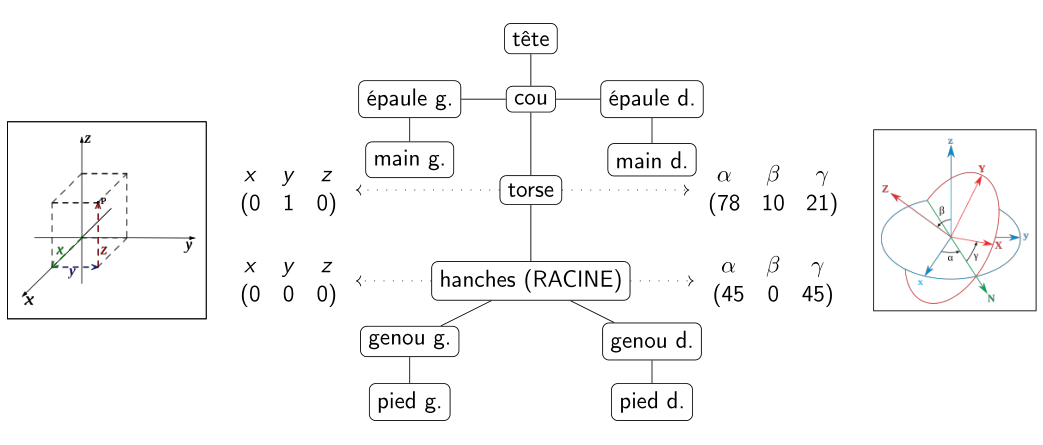
\includegraphics[width=\textwidth]{pictures/skeleton_pos_ori_example.png}
    \caption[Données d'un squelette 3D]{Un exemple de squelette humain représenté sous forme informatique avec, pour chaque articulation, des informations de position et d'orientation relatives à l'articulation parente.}
    \label{fig:skeleton_pos_ori_example}
\end{figure}

Cette structure est particulièrement adaptée pour modéliser tout ou une partie du corps. La représentation du corps humain sous forme de chaîne articulaire 3D, afin de représenter un mouvement, sera celle utilisée dans la suite de ce manuscrit.

% Il existe d'autres représentations pour un corps humain, telle que celle proposée par \parencite{Kulpa2005Mir} : dans ce cas, certains segments du corps sélectionnés sont stockés sous une forme normalisée, ainsi que les plans contenant les articulations intermédiaires non conservées. Cette approche permet une certaine liberté quant à l'adaptation du squelette initial à une autre morphologie, tout en conservant une représentation proche de la réalité du mouvement d'origine. [JUSTIFIER VOIR CORRECTIONS] Seules les données de mouvement représentées sous forme de chaîne articulaires 3D seront considérées dans la suite de ce manuscrit.

Afin d'obtenir un mouvement représenté sous forme d'un arbre, et ainsi exploitable à l'aide d'outils informatiques, il faut être en mesure de le capturer. La capture de mouvements peut être réalisée à partir de plusieurs dispositifs, permettant soit d'obtenir des données 2D (\textit{i.e.} images ou vidéos), ou directement des données 3D (squelette de la personne, nuage de points, modèles surfaciques, \textit{etc.}). En fonction du matériel de capture utilisé, le processus d'acquisition, ainsi que les contraintes associées, la qualité des données obtenues ne sera pas la même. Le choix d'un dispositif de capture adapté à un contexte d'apprentissage de geste doit se faire en fonction des besoins d'observation et d'analyse du geste, tout en prenant en compte les contraintes imposées par la réalisation du geste : amplitude, parties du corps impliquées, manipulation d'objet, environnement spécifique, \textit{etc.}.

\section{Matériel de capture et données obtenues}
Il est possible de séparer l'apprentissage de gestes en deux grandes familles non exclusives : les cas où le geste est la finalité de l'apprentissage, et le cas où la manipulation d'un objet est l'objectif final. Dans le premier cas, le corps humain (une partie ou dans son entièreté) va être au cœur de l'analyse, alors que dans le deuxième cas, la position de l'objet, et parfois le geste permettant d'y arriver seront les points d'intérêt principaux. Les dispositifs utilisés sont ainsi choisis en fonction de l'objet considéré pour la captation (\textit{i.e.} le corps ou un objet), mais aussi du rapport coût/caractéristiques souhaités de l'équipement, déduits de la situation d'apprentissage et des besoins d'observation. En termes de caractéristiques, l'encombrement, l'espace de travail, la chaine de traitements des données et leur précision, ainsi que les retours sensoriels souhaités du système (visuels et/ou haptiques) sont souvent considérés pour ce choix \parencite{Chamaret2010}. Cette section s'intéresse d'abord aux dispositifs dédiés à la capture d'un corps humain, puis aux dispositifs dédiés à la simulation ou la capture de position et d'orientation d'objets. Les coûts de ces dispositifs peuvent être très importants, mais il est maintenant possible d'obtenir des données de mouvements capturés d'une qualité suffisante pour effectuer des analyses de geste d'apprenant à partir de systèmes relativement peu onéreux. Cet aspect \textit{low/middle-cost} de la captation de mouvement est intéressant pour des captures prenant place dans des situations variées (par opposition à la captation dans un environnement dédié, par exemple en laboratoire), ce qui en fait le choix retenu pour cette thèse.

Dans des domaines tels que le sport \parencite{YAMAOKA2013912} (lancer de disque) \parencite{Yoshinaga2015Doa} (archérie) \parencite{Chan2011} (danse), le corps entier de l'apprenant va être capturé et utilisé. Dans ces cas-ci, l'analyse va concerner le mouvement d'une partie ou du corps entier. Il est possible d'obtenir ces données à partir de vidéos, de caméras RGB-D (\textit{Red Green Blue Depth}) \parencite{Yoshinaga2015Doa} \parencite{Kora20151559} \parencite{YAMAOKA2013912}, d'un ensemble de capteurs réduit placés à des endroits spécifiques du corps \parencite{PORCIUNCULA2018S220} ou d'une combinaison de capteurs \parencite{Chang201379}.

\subsection{Extraction de mouvement par vidéo}
Il est possible d'extraire des données de mouvement à l'aide de vidéos. Ces méthodes reposent sur l'inférence du mouvement à partir d'un ensemble de pixels \parencite{Lv2015CEI}. Il existe une multitude de techniques, et certaines d'entre elles permettent d'obtenir un squelette 3D. Une revue des principales méthodes utilisées est proposée dans \parencite{Sarafianos2016DHp} : projection dans un espace 2D de données de mouvement 3D, afin d'obtenir une correspondance avec l'image / la vidéo, utilisation de contraintes rigides sur plusieurs images successives afin de retrouver le squelette le plus probable, \textit{etc.} Il est également possible d'utiliser des vidéos stéréos, permettant ainsi d'obtenir des points de repère dans l'espace et de faciliter le suivi de points spécifiques du corps, afin de reconstituer un squelette 3D correspondant au mouvement (Fig. \ref{fig:stereo_video_skeleton}) \parencite{Liu2016Tb3}.

\begin{figure}[h]
    \centering
    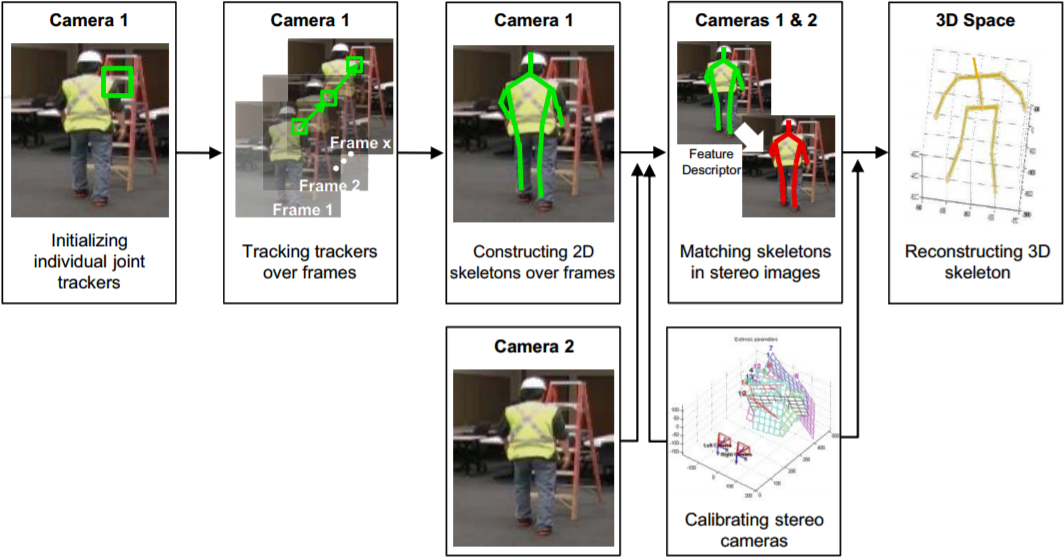
\includegraphics[width=10cm]{pictures/stereo_video_skeleton.png}
    \caption[Squelette reconstitué à partir de vidéo stéréo \parencite{Liu2016Tb3}]{Le squelette 3D peut être reconstitué à partir de vidéo stéréo \parencite{Liu2016Tb3}.}
    \label{fig:stereo_video_skeleton}
\end{figure}


\subsection{Extraction de mouvement par vidéo et capteur de profondeur}
Les caméras RGB-D sont des dispositifs de capture se basant sur la combinaison d'une capture vidéo 2D et d'un mapping de profondeur sur chaque pixel, généralement obtenu à l'aide d'un capteur infrarouge. L'ajout de l'information de profondeur à la vidéo 2D permet d'obtenir une information supplémentaire notamment sur le déplacement des acteurs dans la scène filmée. Leur encombrement relativement réduit, combiné à la non nécessité d’avoir des marqueurs équipés sur le corps font que ces dispositifs ont été largement utilisés dans des contextes de recherche tels que : la capture en temps réel de multiples personnes \parencite{Basso2013}, la reconstruction de scènes interactives en 3D \parencite{Izadi11kinectfusion} ou encore la capture du mouvement \parencite{Yoshinaga2015Doa}. En effet, il est possible d'obtenir le squelette d'une personne à l'aide des outils fournis par les entreprises développant ces caméras (Fig.\ref{fig:skeleton_kinectv2}) : jusqu'à 6 squelettes de 20 articulations chacun peuvent être capturés simultanément (25 articulations par squelette pour la Kinect v2, voir Fig. \ref{fig:skeleton_kinectv2}). La précision de la Kinect permet de capter les pouces de chaque main, mais pas les doigts pris individuellement.\\

\begin{figure}
    \centering
    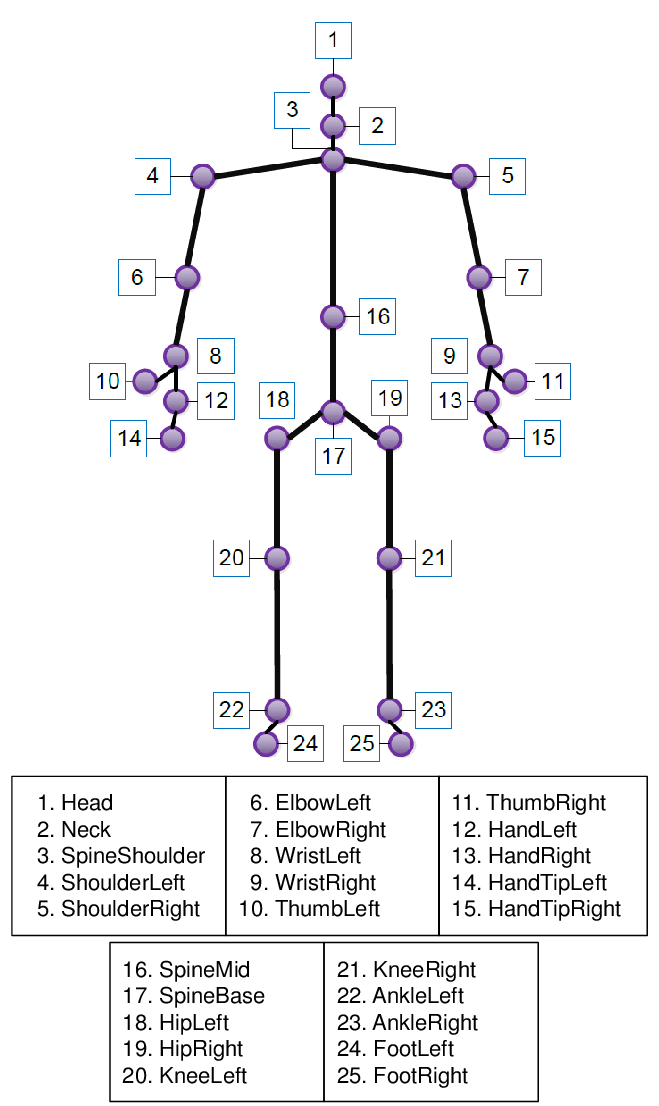
\includegraphics[width=5cm]{pictures/3D-skeleton-joints-tracked-by-the-Kinect-v2-sensor.png}
    \caption[Squelette et articulations captés par la Kinect V2 \parencite{Faisal2015Kinect}]{Squelette et articulations captés par la Kinect V2 \parencite{Faisal2015Kinect}. Le nombre d'articulation est suffisant pour pouvoir représenter les changement de position et d'orientation de tous les membres du corps humain.}
    \label{fig:skeleton_kinectv2}
\end{figure}


Les caméras RGB-D possèdent cependant des inconvénients. En effet, le problème de l'occlusion est fréquent. Il apparaît dès lors qu'une partie du corps est masquée par une autre, par rapport à l'objectif de la caméra. Il est possible de pallier ce problème grâce à l'utilisation de plusieurs caméras en simultanées (Fig. \ref{fig:multiple_rgb_d_camera_system}), et dont les différentes images sont utilisées pour reconstruire le squelette final \parencite{Regazzoni2014Rcv}. Cette méthode nécessite un calibrage très précis, ainsi qu'un environnement dédié à la captation des mouvements.\\

\begin{figure}[h]
    \centering
    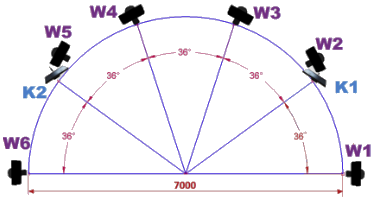
\includegraphics[width=7.5cm]{pictures/multiple_rgb_d_camera_system.png}
    \caption[utilisation de multiples caméras RGB et RGB-B pour éviter l'occlusion \parencite{Regazzoni2014Rcv}]{L'utilisation de plusieurs caméras RGB, ainsi que RGB-D permet d'éviter les problèmes d'occlusion \parencite{Regazzoni2014Rcv}.}
    \label{fig:multiple_rgb_d_camera_system}
\end{figure}

\subsection{Extraction de mouvement par caméra infrarouge}
La méthode la plus précise, en termes de qualité des données, pour capturer un corps entier à l'heure actuelle est celle basée sur les caméras infrarouges utilisées conjointement avec des marqueurs réfléchissants (Fig. \ref{fig:infrared_camera_Morel}). Ces systèmes sont les plus précis pour l'acquisition de mouvements d'une ou plusieurs personnes en simultané \parencite{Pfister2014Cao} \parencite{Yang2016HUL}. Ils sont très utilisés dans l'industrie du cinéma et du jeu vidéo, afin de proposer des mouvements les plus fidèles possibles. Les inconvénients majeurs de ces systèmes sont d'une part le coût (chiffré en plusieurs centaines de milliers d'euros pour un système basé sur 8 caméras), la non portabilité du matériel de capture (nécessité d'avoir un emplacement dédié et fixe) et la chaine lourde de traitements pour reconstituer le squelette 3D (\textit{e.g.} capture des points, filtrage pour la réduction des phénomènes occlusions, reconstitution de la chaîne articulaire et des orientations de chaque articulation). Bien que des entreprises proposent des solutions tout-en-un pour obtenir le squelette 3D d'un ou plusieurs acteurs (\textit{e.g.} Qualysis, Vicon, Optirak), ils nécessitent les compétences d'un informaticien qualifié pour être utilisé. En effet, le placement des capteurs doit se faire de manière optimale (soit en suivant les recommandations fournies par les fabricants des systèmes utilisés, soit en fonction des besoins de captation) afin de s'assurer que les marqueurs réfléchissants soient visibles par au moins une caméra afin de limiter au maximum les phénomènes d'occultation, et les données doivent ensuite être filtrées à l'aide des logiciels fournis par les fabricants ou en utilisant des logiciels externes. Ces filtres peuvent avoir plusieurs objectifs : ré-interpolation du mouvement à une fréquence plus ou moins rapide, lissage des données de mouvement et d'orientation par moyennage des postures proches, effacement des pics de valeurs en fonction des valeurs voisines, \textit{etc.}

\begin{figure}[h]
    \centering
    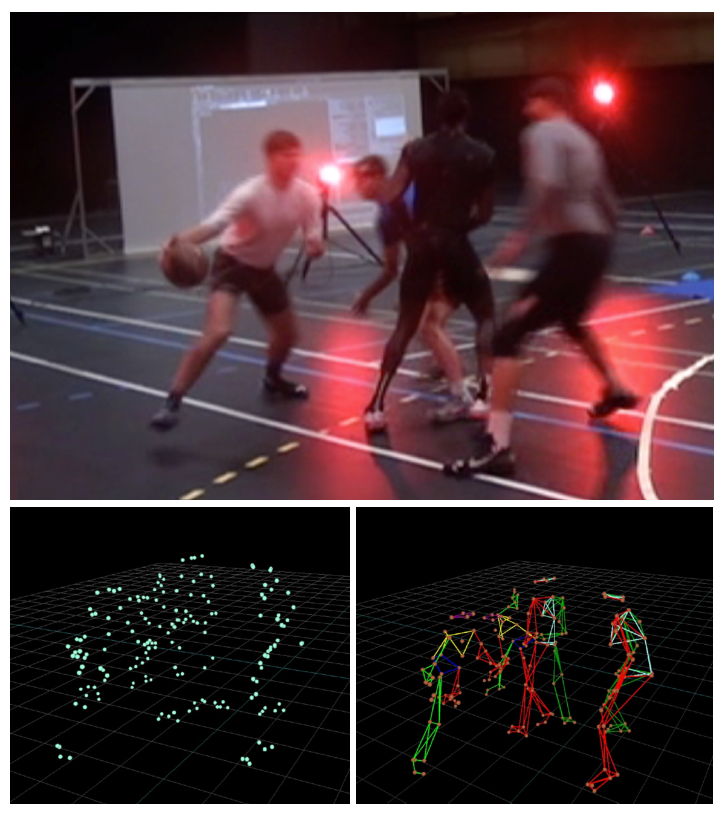
\includegraphics[width=10cm]{pictures/infrared_camera_Morel.png}
    \caption[Système de captation par caméra infrarouge \parencite{Morel2017Mts}]{Un système de captation à base de caméras infrarouges et de marqueurs disposés sur le corps (eu haut). Les données sont obtenues sont la forme d'un nuage de point (en bas à gauche), à partir desquels les squelettes sont reconstitués (en bas à droite) \parencite{Morel2017Mts}.}
    \label{fig:infrared_camera_Morel}
\end{figure}

\subsection{Extraction de mouvement par capteurs inertiels portables}
L'utilisation de capteurs portés par le corps représente une autre méthode pour enregistrer les mouvements. Ces capteurs sont généralement reliés entre eux, et permettent de transmettre les données par une liaison filaire ou sans fil, se libérant ainsi des contraintes de l'espace fixe \parencite{PORCIUNCULA2018S220}. Un capteur renferme un ou plusieurs dispositifs de mesure tels que : un accéléromètre, permettant de mesurer l'accélération linéaire, un gyromètre, permettant de mesurer la vitesse angulaire, et un magnétomètre, qui permet de mesurer la force et la direction d'un champ magnétique. La combinaison de ces trois informations permet de déduire les positions et orientations d'un corps en mouvement dans l'espace. Ainsi, il est possible d'obtenir des données de mouvements dans des contextes plus variés que les systèmes nécessitant une installation fixe. Afin de permettre l'acquisition d'un squelette humain, il est possible de combiner plusieurs de ces capteurs, posés sur plusieurs parties du corps (au niveau des articulations).

Cependant, les données obtenues peuvent être moins précises qu'avec des systèmes fixes (\textit{e.g.} perturbations liées à l'environnement, qualité de transmission des données variable, \textit{etc.}). Un des problèmes souvent rencontrés est celui de la dérive. Il s'agit de la variation des données renvoyées par un capteur, sans que cette variation ne soit le résultat d'un changement de position ou d'orientation réel. Bien que des méthodes existent pour corriger ces défauts, cela implique généralement d'utiliser d'autres types de données pour compenser les erreurs propres au matériel (données GPS, par exemple \parencite{Bevly2004Gps}). Cependant, en fonction du degré de précision nécessaire, ces méthodes ne sont pas toujours adaptées et réutilisables dans tous les contextes. Ainsi, il est parfois nécessaire de disposer d'une chaîne de traitements adaptée afin d'éliminer ces erreurs. Ainsi, une technique de filtrage des données proposée par Roetenberg \textit{et al.} est celle basée sur un filtre de Kalman, fusionnant plusieurs informations provenant de capteurs différents (gyroscopes, accéléromètres, magnetomètres) afin d'estimer l'erreur et ainsi la corriger à la volée  \parencite{Roetenberg2005Com}. Les casques de réalité virtuelle récents font également usage de capteurs inertiels (disposés sur le casque lui-même) afin de proposer une plus grande immersion dans les jeux, en rajoutant le mouvement comme interaction,. L'ajout de ces capteurs inertiels permet également de réduire les problèmes de nausées propres à ces casques \parencite{HTCViveSpecs}.

\subsection{Matériel de captation pour la manipulation d'objets}
Dans le cas où la manipulation de l'objet est au cœur de l'apprentissage, bien que le geste soit parfois important, l'état de l'objet (position, orientation, intégrité, \textit{etc.}) est l'objectif de l'apprentissage du geste, et donc de la captation. Cette différence se retrouve notamment au niveau des données capturées et utilisées : dans les domaines tels que la chirurgie \parencite{BMT_2015} \parencite{Choi2015103} ou la musique \parencite{Ng2008}, la position de l'objet est souvent la donnée de mouvement principale récupérée pendant la tâche (possiblement utilisée conjointement avec d'autres informations, telles que la position du regard \parencite{BMT_2015}). Ces données peuvent être capturées à l'aide de dispositifs adaptés : les interfaces haptiques en sont un exemple (Fig. \ref{fig:haptic_arm}).

Ces interfaces permettent non seulement une manipulation plus aisée d'un objet virtuel, mais également un retour sensitif au niveau du toucher lors de la manipulation \parencite{SREELAKSHMI20174182}. Ainsi, il est possible d'obtenir des retours de force ou tactile permettant d'émuler respectivement la forme ou la texture d'un objet. En combinant ces retours à des environnements de réalité virtuelle, il est possible de proposer une sensation de saisie, de collision et de toucher, en conjonction avec ce qui est visuellement présenté à l'utilisateur \parencite{Whitmire2018}. Ce dispositif est très utilisé dans le cadre de l'apprentissage de manipulation d'objets médicaux, tels que pour l'insertion d'aiguilles sous la peau \parencite{CORREA20196}, la manipulation de sondes \parencite{Choi2015103}, le cathétérisme \parencite{PEPLEY20171066}, ou encore l'entrainement du personnel à la planification pré-opératoire par télé-chirurgie \parencite{HALABI20189}.

\begin{figure}
    \centering
    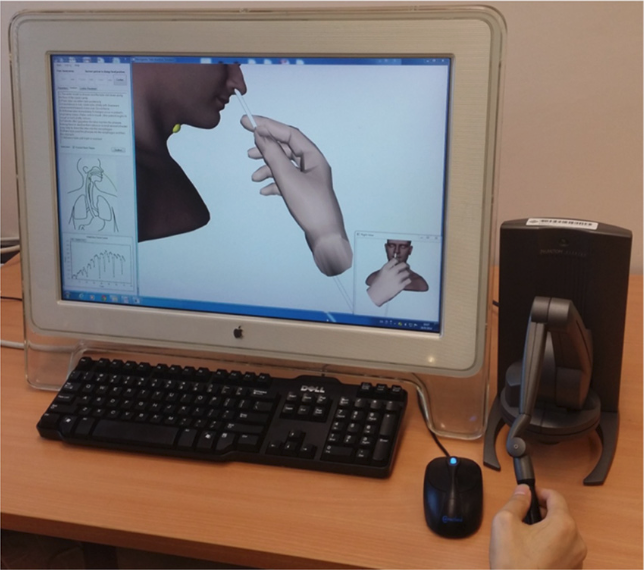
\includegraphics[width=7.5cm]{pictures/haptic_arm.png}
    \caption[Bras haptique simulant l'insertion d'une sonde naso-gastrique \parencite{Choi2015103}]{Exemple de bras haptique servant à simuler l'insertion d'une sonde naso-gastrique, avec un modèle 3D mis à jour en temps réel à côté \parencite{Choi2015103}.}
    \label{fig:haptic_arm}
\end{figure}

Par exemple, dans le cadre de la simulation de l'insertion d'une sonde naso-gastrique, Choi \textit{et al.} ont utilisé un modèle physique 3D de tête humaine conjointement avec un bras haptique \ref{fig:haptic_arm} \parencite{Choi2015103}. Ce système permet de générer la sensation d'une insertion et de buttée si jamais la sonde touche une partie de la gorge, et ainsi de pouvoir ajuster le geste en temps réel.

Dans le domaine industriel, Chamaret \textit{et al.} ont capturé des mouvements à l'aide d'un dispositif appelé « spidar » \parencite{Chamaret2010}. Le but était d'étudier et d'évaluer différentes procédures d'assemblage et de démontage d'un phare de voiture, dans un environnement virtuel. Les modèles 3D, ainsi que le retour de force, étaient adaptés à la morphologie de l'utilisateur. L'objectif était d'évaluer empiriquement la capacité de l'utilisateur à accomplir la tâche demandée, en accord avec le nombre de collisions.\\

Les dispositifs haptiques disposent souvent d'un espace de travail limité (bras à retours d'efforts), contraignant l'utilisateur dans ses mouvements à cet espace (bras à retour d'effort à socle fixe) ou par le poids de ces dispositifs (veste tactile, bras à retours d'efforts portatifs, gants à retour d'efforts).  Cependant, les situations d'apprentissage du geste ne se limitent pas toujours à un espace de travail restreint. Dans le contexte de l'apprentissage de gestes sportifs ou artistiques par exemple, le corps ainsi que les objets manipulés peuvent évoluer dans un espace 3D avec un volume/espace de travail conséquent.

Dans ces cas, plusieurs méthodes de suivi de l'objet existent. L'une d'elles utilise des marqueurs réfléchissants placés sur l'objet à suivre, afin d'en obtenir la trajectoire dans l'espace et le temps, au même titre que les méthodes vues précédemment servant à capter le corps d'un humain. Le positionnement de ces capteurs sur l'objet en question (Fig. \ref{fig:markers}) doit faire l'objet d'une attention particulière, afin de limiter les problèmes d'occlusion. Shapira \textit{et al.} utilisent un ensemble de caméra infrarouges combinées à des casques de réalité virtuelle et des objets (des cubes mous et des jouets divers) équipés de de sphère réfléchissantes, afin d'être captées et utilisées au sein de l'environnement virtuel \parencite{Shapira2016TVR}. Un autre test en utilisant des bâtons réfléchissants à la place des sphères a été réalisé, cependant, les objets étant manipulés par des enfants, ces marqueurs étaient le plus souvent occultés par ces derniers. Ainsi, les sphères réfléchissantes positionnées sur les arrêtes des objets à manipuler se sont révélées plus efficaces pour réussir à suivre les déplacements et rotations des objets dans l'espace.

\begin{figure}
    \centering
    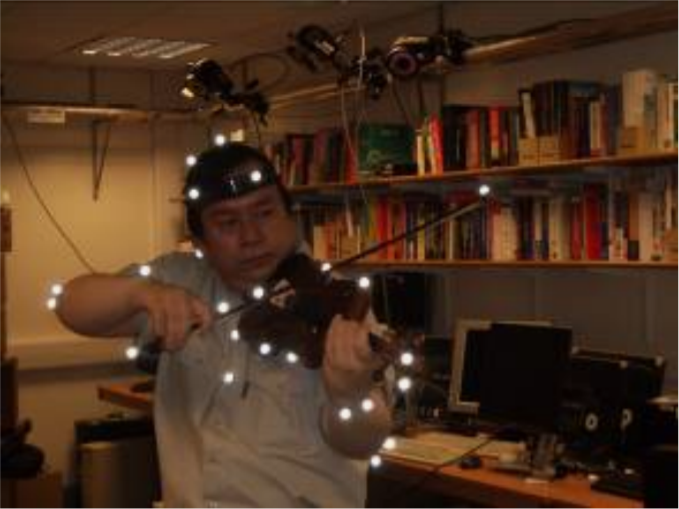
\includegraphics[width=7.5cm]{pictures/markers.png}
    \caption[Marqueurs réfléchissants sur une personne et un objet \parencite{Ng2008}]{Exemple de marqueurs réfléchissants positionnés sur une personne et un objet \parencite{Ng2008}.}
    \label{fig:markers}
\end{figure}

%Dans le cadre de l'apprentissage du violon, des capteurs réfléchissants placés sur l'archet et le corps du violon ont été utilisés dans \parencite{Ng2008}, afin de suivre sa position dans le temps et l'espace. Ces capteurs, d'une taille d'un centimètre de diamètre, étaient captés par 12 caméras infrarouge disposées autour de la personne réalisant le mouvement, afin de minimiser au maximum la perte de tracking d'un des capteurs à cause d'une occlusion. La position des marqueurs sur l'instrument était également susceptible de gêner le mouvement du violoniste. Pour pallier ce problème, un modèle statique de l'instrument ayant tous les marqueurs nécessaire à la captation du violon a été créé, puis un modèle avec moins de marqueurs a été utilisé pour le jeu, le modèle final du violon étant reconstruit en calculant les positions des marqueurs manquants par rapport au modèle statique.\\

\subsection{Bilan sur les dispositifs de captation de mouvement}
La qualité des données produites par les différentes méthodes d'acquisition peut varier grandement, notamment à cause des problèmes spécifiques aux matériels utilisés (problèmes d'occlusion pour les caméras RGB-D, problème de dérive pour les capteurs inertiels portés). Cependant, les matériels de captation fournissant les données plus précises possèdent un coût d'achat parfois prohibitif, ainsi qu'une mise en place plus contraignante. De plus, ils nécessitent parfois l'utilisation d'une chaîne de traitement (intégrée aux logiciels fournis avec système de capture ou non) afin d'obtenir des données exploitables. Concernant les systèmes moins coûteux, tels que la captation à l'aide de caméras \textit{RGB-D} ou de combinaison de capteurs inertiels, la mise en place du matériel est moins contraignante (en terme de temps et d'espace), et nécessite moins de traitements afin d'obtenir des données utilisables. Quelle que soit l'utilisation faite du mouvement, il faut être en mesure de disposer de données non-bruitées par les systèmes de capture. Les systèmes au sein desquels sont utilisées des données de mouvement doivent souvent intégrer une chaine de traitements du mouvement, soit pour le filtrage, soit pour l'extraction d'informations sur une partie précise du mouvement global. Ce besoin est crucial dans les systèmes dédiés à l'apprentissage de mouvements, indépendamment du contexte applicatif.

Dans le contexte de la thèse, la captation par combinaison de capteurs inertiels a été retenue. Plus précisément, il s'agit de la combinaison Perception NEURON. L'installation et la calibration d'une telle combinaison est rapide, et elle n'encombre que marginalement la personne la portant. La possibilité d'utiliser de tels dispositifs sans être contraint à un espace de travail fixe permet de mieux s'adapter au contexte du geste à effectuer (contraintes d'environnement, d'espace nécessaire, \textit{etc.}). Le logiciel fourni, servant à récupérer les informations transmises par la combinaison, intègre une série de pré-traitements, afin de filtrer les données de mouvement obtenues. Les retours proposés par le système se basant sur le mouvement seul, et étant donnés par un expert ou le système lui-même, il n'y a pas besoin d'utiliser un système de retours haptiques. Enfin, le coût faible d'une telle combinaison par rapport aux systèmes de captation plus perfectionnés est des atouts dans le contexte d'un EIAH permettant d'aider à l'apprentissage de geste qui se veut utilisables par tous.

%\section{Nombre de données}
%Dans un contexte informatique, plusieurs stratégies existent pour améliorer l'apprentissage du geste. Ainsi, au même titre que le type des données peut être différent, la quantité utilisée peut l'être également.

%L'utilisation d'un squelette 3D d'expert reproduisant le mouvement est une manière d'apprendre le mouvement analogue aux techniques se passant d'outils informatique.

%L'utilisation de modèles experts mis en parallèle avec celui de l'apprenant est une piste qui a été exploré dans l'apprentissage du geste \parencite{Yoshinaga20151497} \parencite{Kora20151559}. Dans ce cas, le geste de l'expert est enregistré, et est rejoué à côté de celui de l'apprenant, ou en les superposant. Le systèmee proposé par \parencite{Yoshinaga20151497} se base sur plusieurs modèles d'experts, à partir desquels il est possible d'obtenir un expert " moyen " (\textit{i.e.} une moyenne des modèles experts), l'expert médian, ou celui le plus proche de l'apprenant en terme de morphologie.


%La superposition virtuelle du mouvement de l'apprenant et de celui de l'expert est une piste qui a été exploré dans l'apprentissage du geste. Dans le domaine de l'archerie japonaise, Yoshinaga et Soga ont développé un système basé sur une caméra RGB-D (Kinect), afin de capturer le mouvement de l'apprenant \parencite{Yoshinaga20151497}. Dans ce système, des mouvements d'experts ont été préalablement capturés à l'aide d'une caméra RGB-D (Kinect), permettant ainsi à l'apprenant de se comparer avec les modèles experts. Le modèle choisi peut être celui d'un expert en particulier, ou une combinaison (moyenne) des modèles, ou encore le modèle étant le plus proche morphologiquement de l'apprenant. Ce système nécessite donc la capture d'un certain nombre d'experts, pour proposer une large gamme de morphologies. L'analyse est ici empirique, effectuée soit par un expert, soit par l'apprenant lui-même en observant la superposition des deux gestes. Kora \textit{et al.} ont utilisés de nombreux dispositifs (casque de réalité virtuelle avec caméra, Kinect. \textit{etc.}) afin de construire un système d'apprentissage du golf \parencite{Kora20151559}. Grâce à la superposition du squelette de l’apprenant et du squelette de l’expert, l’utilisateur est capable de voir son mouvement en temps réel, et ainsi essaye de coller au mieux au mouvement expert. Cependant, cet affichage en temps-réel peut être perturbant et aucune information pédagogique n’est extraite de ce processus. Yamaoka \textit{et al.} propose un système permettant de capturer le mouvement de l'apprenant et de lui donner un retour sur sa performance, dans le contexte du lancer de disque \parencite{YAMAOKA2013912}. Les données sont capturées à l'aide d'une caméra RGB-D (Kinect), puis le mouvement est segmenté en 3 parties, correspondant à la phase de pré-mouvement, mouvement, et post-mouvement. Ces phases sont extraites automatiquement, en observant la position relativement des articulations entre elles, et en segmentant quand un seuil est dépassé. Le retour sur le mouvement est donné selon 5 aspects: (a) mouvement arrière suffisant (avant le lancer), (b) hauteur de la main droite suffisante, (c) transition de hauteur de la main droite, (d) angle de l'épaule droite adéquat, (e) rotation de la hanche suffisante. Les consignes données à l'apprenant sont de la forme " Levez votre main droite ", ou encore " votre hanche doit plus tourner ". Les résultats ne montrent pas d'amélioration significative du résultat du lancer avec le système de conseils mis en place. Ng s'est intéressé à l'apprentissage du violon \parencite{Ng2008}. La capture du mouvement s'effectue uniquement sur l'instrument et l'archet, à l'aide de capteurs réfléchissants. La position des différents éléments nécessaire au jeu est ensuite affichée grace à l'interface proposée. L'EIAH développé permet la visualisation des partitions selon le standard ISO MPEG Symbolic Music Representation (SMR), l'écoute du morceau, un système de tracking en temps réel du mouvement de l'apprenant, ainsi que l'écoute du jeu, permettant de donner des conseils et de proposer de " tourner la page " des partitions en temps réel. Le système propose également une analyse des mouvements à l'aide de clustering, afin de détecter automatiquement quel style de jeu est utilisé (\textit{e.g.} tenuto, staccato, spicato, \textit{etc.}).

\section{Environnements informatiques pour l'apprentissage de gestes}
Il existe de nombreux EIAH dédiés au geste. La finalité de l'apprentissage des gestes au sein de ces systèmes est variée : apprentissage actif impliquant d'avantage l'étudiant \parencite{Xu2019Ptt}, rééducation \parencite{Alankus2010TCG} \parencite{Baldominos2015AAt}, amélioration de la performance sportive \parencite{Maes2012DtM}, \textit{etc.} Ces catégories ne sont pas exclusives, et les systèmes développés se retrouvent souvent à l'intersection de plusieurs d'entre elles. Les domaines d'application sont également variés : médical (\textit{e.g.} analyse de postures \parencite{Aminian2004Chm}, chirurgie \parencite{BMT_2015}, etc.), sport (\textit{e.g.} danse \parencite{Maes2012DtM}, archerie japonaise \parencite{Yoshinaga2015Doa}, lancer de disque \parencite{Yamaoka2013FoF}), et les techniques utilisées peuvent également faire appel à la réalité virtuelle, par exemple \parencite{Kyan2015ABD}. Pour chaque EIAH, il est possible d'identifier des caractéristiques qui lui sont propres : domaine d'application, objectif visé de l'apprentissage, objectif visé de la ou des tâches à apprendre, prise en compte des besoin d'observation et fonctionnels de l'enseignant, utilisablitié vis-à-vis de l'usager afin de créer et d'évaluer une nouvelle tâche, type de données utilisées pour l'analyse du geste, méthodes d'analyse, retours faits à l'apprenant, \textit{etc.}  En effet, un EIAH sera efficace et démocratisable si l'usager a été placé au cœur de sa conception afin de : (i) répondre à ses besoins d'observation et fonctionnels, (ii) prouver son utilisabilité et (iii), des modèles génériques de conception ont été extraits afin de minimiser la réingénierie en cas de modification de la tâche, des observations et du domaine d'application. Cette section étudie les principaux EIAHs basés « geste » selon ces caractéristiques.

%Le regroupement de ces caractéristiques permet de mettre en évidence un manque d'EIAH dédiés à l'apprentissage du geste réutilisable dans d'autres contextes sans nécessiter de réingénierie conséquente, à cause d'une dépendance trop forte au matériel ou au domaine applicatif retenu.

\subsection{Quelques exemples significatifs d’EIAH pour apprendre des gestes}
Dans le domaine médical, la rééducation nécessite par exemple la répétition de gestes permettant de renforcer une partie du corps, ou de réapprendre à utiliser un membre. Il est possible de faciliter la répétition de certains de ces gestes à l'aide d'interfaces dédiées. Baldominos \textit{et al.} ont développé un EIAH permettant de faire répéter les gestes requis par le médecin pour la rééducation de parties spécifiques du corps \parencite{Baldominos2015AAt}. Dans cette étude, les exercices sont focalisés sur un travail des adducteurs, ainsi que les abducteurs. La mise en situation proposée est celle d'un gardien de but (Fig. \ref{fig:eiah_baldominos}). L'expert peut intervenir ou non dans la séance de rééducation. Si l'expert est présent, il peut choisir le moment du tir du ballon, la vitesse ainsi que de la hauteur de la balle. Dans le cas d'une session d'apprentissage sans expert, le système commence par effectuer des tirs bas, espacés dans le temps, puis augmente ou diminue l'intensité des deux paramètres (hauteur et temps entre les tirs) en fonction du score du patient. Dans les deux cas, une augmentation progressive de la difficulté de la tâche à effectuer permet d'augmenter l'amplitude du mouvement nécessaire, et ainsi de faire progresser le patient. De plus, l'utilisation de dispositifs tels qu'un casque de réalité virtuelle masque les parties du corps, ce qui demande une concentration accrue afin de synchroniser ses mouvements et d'être capable de se situer dans l'espace. %Cette capacité à percevoir les différentes parties de son corps à l'aide des récepteurs sensoriels musculaires et ligamentaires s'appelle la proprioception, et le travail supplémentaire nécessaire au développement de cette perception augmente l'efficacité du traitement, tout en diminuant sa durée \parencite{Missaoui2009Hfd}.

\begin{figure}
    \centering
    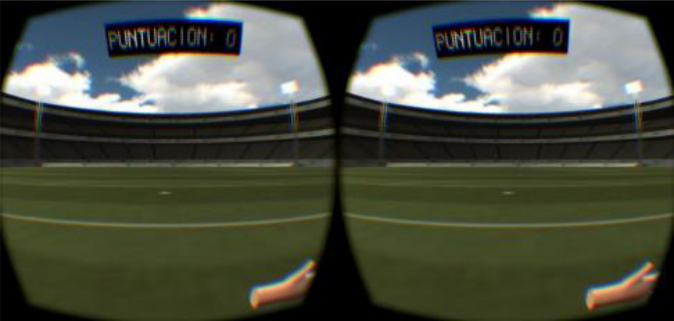
\includegraphics[width=\textwidth]{pictures/eiah_baldominos.png}
    \caption[EIAH pour la rééducation \parencite{Baldominos2015AAt}]{L'environnement de réalité virtuelle proposé par \parencite{Baldominos2015AAt}. La mise en situation dans un cadre crédible par rapport aux exerciecs à effectuer permet d'augmenter l'implication du patient \parencite{Baldominos2015AAt}.}
    \label{fig:eiah_baldominos}
\end{figure}

Les travaux de Alankus \textit{et al.} proposent un système permettant d'engager plus fortement les victimes d'attaque cardiaque lors de la rééducation à domicile \parencite{Alankus2010TCG}. Après une attaque cardiaque, il y a souvent une perte de mobilité de la part du patient. Dans le cadre de la rééducation post-attaque cardiaque, il est souvent nécessaire pour le patient de répéter des gestes, afin de retrouver une certaine mobilité. Ces gestes sont définis par l'expert, en fonction de la gravité des lésions cérébrales et de l'avancée de la rééducation. Bien que les séances avec les spécialistes soient dédiées à ces gestes, la durée, ainsi que la fréquence de ces séances est insuffisante; c'est pourquoi le patient doit également réaliser des gestes répétés chez lui.
%Cependant, seulement un tiers des personnes font suffisamment de répétition de ces mouvements \parencite{Shaughnessy2006TaM}. Ce système offre une motivation supplémentaire à l'aide de la gamification des exercices à réaliser.
Dans ce contexte, les mouvements sont capturés à l'aide de dispositifs communs et abordables : webcam et Wiimote™. Plusieurs jeux ont été développés : déplacement de personnages dans l'espace, jeu de course automobile, lancer et rattrapage de balle de baseball, jardinage (élimination des mauvaises herbes en laissant les fleurs intactes), \textit{etc.} Chacun de ces jeux se concentre sur un mouvement précis à réaliser, allant de mouvement amples (balayage du bras) à des mouvements fins (utilisation de contrôleurs analogiques pour déplacer un personnage). Ils ont été développés en collaboration avec des médecins, afin de solliciter les capacités cognitives du patient, ainsi que les parties du corps concernées par la rééducation. Ils permettent d'activer des parties du cerveau différentes, en stimulant soit la mémoire, le contrôle d'une partie du corps spécifique, la coordination des membres du corps ou les facultés d'anticipation. Le système peut lui-même modifier la difficulté des jeux (et donc l'intensité des exercices), et il est également possible pour l'expert de personnaliser les jeux, afin de les adapter aux différents patients. Par exemple, il peut définir un ensemble de valeurs correspondant à différents niveaux de difficultés, afin que cette difficulté s'adapte au patient pour que l'exercice propose toujours un défi suffisamment élevé afin d'améliorer l'efficacité de la rééducation. Dans le cas du jeu Pong (un des jeux proposés par le système), la taille de raquette et de la balle, ainsi que la vitesse de la balle peuvent être changées.

Lorsque l'objectif est de réussir un geste menant à la manipulation d'un objet,  comme dans le domaine de la chirurgie, le système peut combiner plusieurs types de données hétérogènes, afin d'évaluer plusieurs modalités. Par exemple, le système utilisé par Toussaint  permet de combiner les données de mouvement d'un bras haptique (utilisé pour simuler la manipulation d'un trocard) ainsi que le retour de force associé (simulant les variations de densités du corps humain et des vertèbres), et d'un oculomètre, afin de suivre la trajectoire du regard au cours d'une opération (Fig. \ref{fig:eiah_toussaint}) \parencite{BMT_2015}. Les connaissances mises en jeu sont appelé « perceptivo-gestuelles », car elles combinent la vision et le geste. Un algorithme d'extraction de \textit{patterns}, \textit{PhARules}, inspiré de \textit{CMRules}, permet d'extraire des séquences d'actions en fonction des phases dans lesquelles elles sont réalisées. Les détail du parcours de l'apprenant, ainsi que les interactions pour chaque séquence de l'opération sont fournis. Ces interactions peuvent être de type « contrôle \textit{a priori} » (\textit{e.g.} une observation des signes vitaux du patient avant l'opération), « contrôle \textit{a posteriori} » (\textit{e.g.} une observation des signes vitaux du patient après être intervenu sur le patient) ou « mixte » (\textit{e.g.} prise d'information et manipulation du patient en simultané). Selon le degré de réussite de la procédure, le système propose un retour à l'apprenant : réalisation d'un exercice complémentaire sur un nouveau cas clinique simulé afin de renforcer l'acquisition des connaissances sur un point précis, proposition de révision des cours théoriques, approfondissement de la connaissance du cas clinique qui vient d'être traité.

\begin{figure}
    \centering
    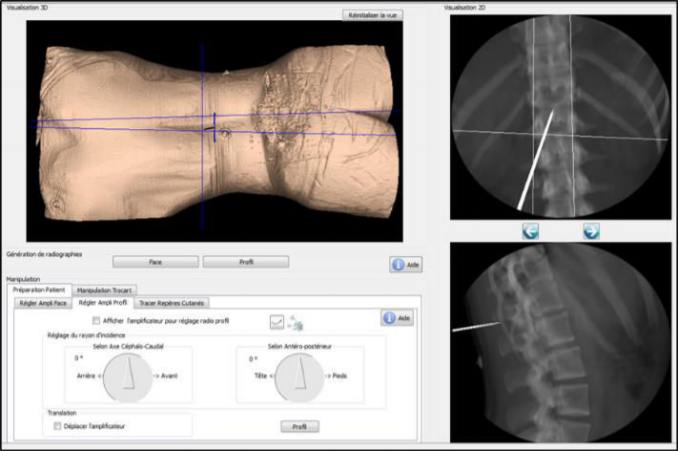
\includegraphics[width=\textwidth]{pictures/eiah_toussaint.png}
    \caption[EIAH pour la chirurgie orthopédique \parencite{BMT_2015}]{Le système utilisé par \parencite{BMT_2015} permet de combiner les données d'un oculomètre ainsi que d'un bras haptique afin de donner un retour couvrant tous les aspects importants d'une procédure chirurgicale orthopédique \parencite{BMT_2015}.}
    \label{fig:eiah_toussaint}
\end{figure}

%Des études telles que Ferrari \textit{et al.} proposent d'intégrer une évaluation des mouvements en contexte industriel par rapport aux normes de sécurité et d'ergonomie \parencite{Ferrari2018MAS}. L'étude se base sur la capture du mouvement, mais également l'analyse de la productivité d'un opérateur d'une part, et d'autre part l'analyse de la posture, de la position et de différentes modalités (telles que la distance effectuée, la vitesse moyenne au cours de l'activité, l'amplitude verticale) pour des articulations précises, en fonction de la tâche à accomplir : mains pour la prise d'objets, haut du corps pour le déplacement du corps, par exemple. Ces travaux se basent sur les méthodes d'évaluation ergonomiques internationales OWAS, REBA, NIOSH et EAWS. Les informations extraites et analysées du mouvement sont le déplacement et la vitesse de certaines parties du corps, les mouvements verticaux dus au soulèvement et la pose d'objets, le chemin suivit de l'opérateur en poste ainsi que la trajectoire de sa main, l'utilisation de l'espace de travail, la fréquence ainsi que la durée des opérations de déplacement d'objet, et la répartition du temps entre les tâches dites à valeur ajoutée (exécution d'une tâche) et les tâches sans valeur ajoutée (marcher, prendre un objet, etc.). Le système est configuré pour un environnement de travail particulier. La connaissance de l'expert est réduite à un ensemble de règles d'ergonomies utilisées. Bien que le système propose une évaluation du mouvement, aucune recommandation supplémentaire n'est fournie par le système quant aux changements à effectuer, tant sur le poste de travail que sur le geste de la personne. Les données fournies par le système doivent être analysées par une personne à même de les mettre en relation avec le poste de travail occupé, afin d'effectuer des changements soit dans le rythme du travail imposé, soit dans la disposition des éléments du poste de travail.

L'apprentissage de la langue des signes est difficile, et nécessite une pratique régulière pour les non-natifs \parencite{Cooper2011Slr}. La captation et l'analyse des gestes de la langue des signes nécessitent de prendre en compte : (i) toutes les parties du corps situées au-dessus du bassin, en tant qu’éléments signifiant du discours et (ii) la précision et la rapidité des mouvements effectués par certaines parties du corps telles que les mains et les doigts \parencite{Gibet2016IEi}. En utilisant des données enregistrées avec un dispositif low-cost (Microsoft Kinect™), le système développé par Gameiro \textit{et al.} permet de faciliter l'apprentissage de la langue des signes grâce à deux modes d'utilisation : le mode « classe », et le mode « compétition » (Fig. \ref{fig:eiah_gameiro}) \parencite{Gameiro2014KST}. Le mode classe met l'apprenant face à une situation d'apprentissage où il doit répéter les signes présents à l'écran, jusqu'à ce que le signe soit correctement fait. Le mode compétition est gamifié, et propose une situation de type quizz télévisé, où le but est de répondre en signant à des questions permettant de tester les connaissances de la personne. L'autre défi du mode compétition consiste en une évaluation des capacités de l'apprenant à épeler et signer correctement un mot, en composant les signes des lettres successives. Dans ce cas, l'évaluation est binaire : soit le geste correspond au signe à réaliser, soit il ne correspond pas. L'évaluation se fait à l'aide d'un masquage des données de l'apprenant par les signes correspondant aux lettres à signer présents dans la base de données. Bien que présentant des résultats positifs avec des classes d'étudiants en langage des signes, les auteurs notent que la reconnaissance automatique des signes de l'apprenant est meilleure lorsque la base de données de signes de référence est construite à partir des mouvements de l'apprenant. Cela s'explique par les différences morphologiques entre les différentes personnes ayant utilisé le système, à cause de l'absence de normalisation ou de mise à l'échelle des données capturées par la caméra.

\begin{figure}
    \centering
    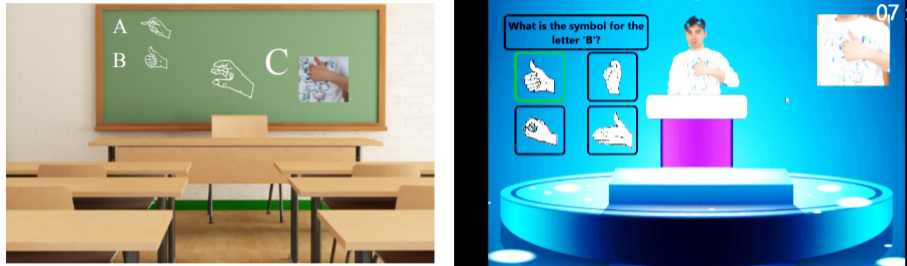
\includegraphics[width=\textwidth]{pictures/eiah_gameiro.png}
    \caption[EIAH pour l'apprentissage de la langue des signes \parencite{Gameiro2014KST}]{Le système proposé par \parencite{Gameiro2014KST} met d'une part l'apprenant dans une situation classique d'apprentissage (à gauche), puis permet de tester les connaissances à l'aide d'une gamification type " quizz télévisé " (à droite) \parencite{Gameiro2014KST}.}
    \label{fig:eiah_gameiro}
\end{figure}

L'EIAH développé par Xu \textit{et al.} permet de faire apprendre à des enfants certains gestes, complexes ou non \parencite{Xu2019Ptt}. Dans cette étude, ces gestes étaient liés à la culture Chinoise : manipuler un métier à tisser, tirer à l'arc, chevaucher un cheval, manipuler des panneaux, \textit{etc.} Les gestes sont acquis à l'aide d'une caméra \textit{RGB-D}. Le mouvement est segmenté dans un premier temps, à l'aide d'un modèle de Markov caché, comparant le mouvement complet de l'apprenant à plusieurs combinaisons de mouvements issus de la base de données de mouvements à effectuer. La combinaison de mouvements ayant la plus grande similitude avec les gestes de l'apprenant est choisie comme modèle du geste réalisé par l'apprenant, et le découpage du mouvement de l'apprenant s'effectue selon cette combinaison. La comparaison du geste de l'apprenant à celui à effectuer intervient à la suite de la segmentation, et est également réalisée par un modèle de Markov caché, à l'aide plusieurs modules permettant chacun de reconnaître un geste. Ainsi, en décomposant le mouvement en plusieurs parties, il est possible de comparer chaque étape d'un geste continu aux gestes cible présents dans la base de données de gestes, et donc de déterminer si le geste est réussi ou non. S'il ne l'est pas, le système va proposer un exercice permettant de se focaliser sur la ou les parties du geste ratées, à l'aide d'un autre modèle de Markov caché (Fig. \ref{fig:eiah_xu}). Ce réseau se base sur les résultats de l'analyse des gestes du précédent : ainsi, en chaque point où le geste de l'apprenant n'est pas conforme au geste attendu, le système va être en mesure de proposer plusieurs ressources différentes (explications textuelles, vidéo de démonstration, \textit{etc.}) pour expliquer ou montrer à l'apprenant quel est le geste attendu. Par exemple, dans le cas de la manipulation du métier à tisser, le système peut détecter si l'apprenant ne regarde pas le métier à tisser pendant la tâche, ou si la distance entre son corps et le métier à tisser est trop grande, et lui faire visualiser une vidéo lui montrant la posture à adopter pour réaliser cette tâche. L'apprentissage du geste est ainsi amélioré en faisant répéter des parties spécifiques à l'apprenant, avant de passer à la suite du parcours. De cette manière, il est possible de mettre l'accent sur les mouvements que l'apprenant a du mal à réaliser.

\begin{figure}
    \centering
    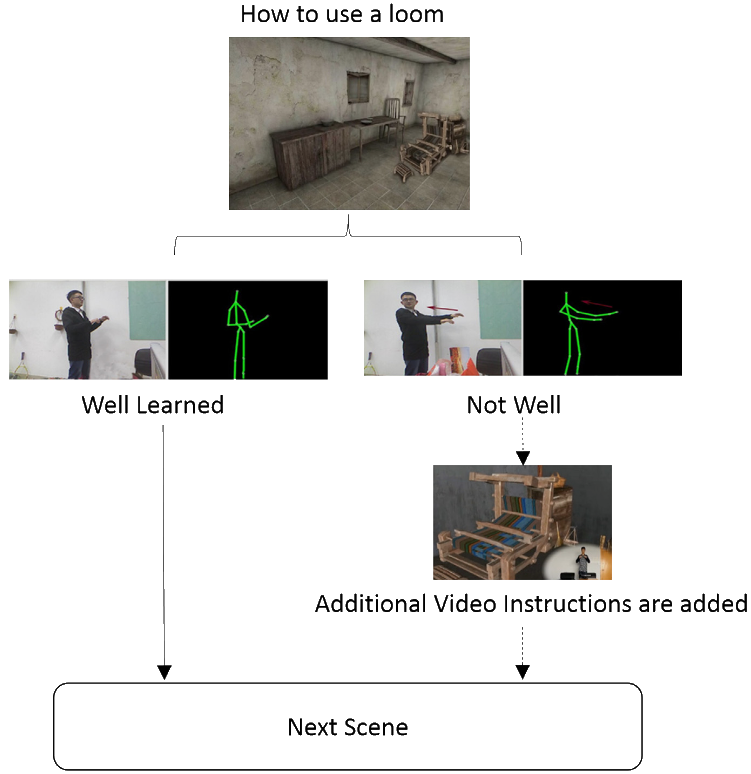
\includegraphics[width=7.5cm]{pictures/eiah_xu.png}
    \caption[EIAH permettant de corriger des parties spécifiques du geste \parencite{Xu2019Ptt}]{L'adaptation du parcours d'apprentissage proposé par Xu \textit{et al.} permet de corriger des parties spécifiques du mouvement de l'apprenant \parencite{Xu2019Ptt}.}
    \label{fig:eiah_xu}
\end{figure}

Le domaine artistique et sportif fait usage des EIAH pour l'apprentissage de gestes. Chan \textit{et al.} ont développé un système permettant d'apprendre des mouvements de danse, en se basant sur des données de mouvement d'expert enregistrées au préalable à l'aide d'un système basé sur une combinaison de capteurs réfléchissants et des caméras infrarouge, afin de l'afficher sur un écran \parencite{Chan2011}. En observant les gestes de l'expert, l'apprenant le reproduit ensuite, et ses données sont capturées, afin d'être comparées à celles de l'expert. Les données sont stockées sous forme de squelettes 3D, à partir desquels plusieurs analyses sont faites. Dans ce système, les différences morphologiques entre l'apprenant et l'expert sont atténuées à l'aide d'une normalisation des positions des articulations par la somme des membres du corps. Plusieurs retours sont offerts à l'apprenant. En premier lieu, une visualisation en temps réel du mouvement de l'expert et de celui de l'apprenant est proposée, en colorant les différentes parties du corps de l'apprenant en fonction des différences avec le geste de l'expert (lorsqu'un certain seuil de distance est franchi entre les positions des articulations de l'expert et de l'apprenant). Il est également possible de rejouer le mouvement au ralenti, afin de mieux voir les différences entre les gestes. Enfin, un score de performance global, correspondant à la somme des distances des articulations de l'apprenant par rapport à celles de l'expert, est fourni à l'apprenant.

Le système d'aide à l'apprentissage de la danse développé par Maes \textit{et al.} propose une approche différente pour la visualisation des mouvements de l'expert \parencite{Maes2012DtM}. Trois étapes sont proposées : la visualisation du mouvement réalisé par l'expert, l'apprentissage en réalisant le geste de manière décomposée afin d'apprendre chaque étape, et l'évaluation à l'aide d'un score indiquant la performance de l'apprenant. La décomposition du mouvement est réalisée de manière automatique, en analysant d'une part le rythme et le tempo de la musique, et d'autre part le mouvement de l'expert réalisant le geste. Les points d'inflexions dans ces valeurs synchronisées avec les tempos sont utilisés comme séparateurs du mouvement. L'expert peut ensuite valider cette séparation avant d'intégrer le geste au système. Le score se base sur le coefficient de corrélation croisée de Pearson entre les données de mouvement de l'expert et celles de l'apprenant, un score de 1 indiquant une similitude parfaite entre les deux gestes, alors qu'un score de 0 indique une dissimilitude complète. L'utilisation de systèmes intégrant un tuteur intelligent (souvent appelés « coachs ») permet de s'affranchir de la présence d'un expert, et donc de l'obligation de se rendre dans un endroit spécifique pour pratiquer, et permet également d'entraîner des personnes en parallèle. Dans ces systèmes, l'expert n'intervient que dans l'enregistrement et l'intégration des données au système, le retour à l'apprenant est fait par le système à l'aide d'un score ou de conseils par exemple.

Dans le domaine du sport, il est également possible de développer de tels systèmes pour la découverte automatique de la différence entre le geste d'un expert et d'un débutant, comme le système proposé par Makio \textit{et al.}, servant à séparer les gestes de service au tennis des professionnels de ceux des amateurs \parencite{Makio2007DoS}. Dans ce cas, le système permet d'extraire dans un premier temps des règles d'associations entre les différentes parties du corps, afin de découvrir les mouvements effectués par l'expert. Dans un premier temps, le mouvement est segmenté à partir des points où la vitesse (sur un des trois axe) d'une articulation spécifiée est égale à zéro. Les parties du mouvement ainsi segmentées sont ensuite comparées entre elles à l'aide du Dynamic Time Warping (DTW), afin d'obtenir un score de similitude. Les mouvements sont ensuite regroupés à l'aide d'un algorithme de clustering, afin de réunir au sein d'un même groupe plusieurs sous-parties du mouvement correspondant au même geste. L'utilisation de deux fenêtres glissantes, l'une active (correspondant aux mouvements ayant une influence sur d'autres mouvements) et l'autre passive (correspondant aux mouvements étant influencés par d'autres mouvements) permet ensuite de détecter les dépendances récurrentes entre les parties du corps lors de la réalisation d'un geste, correspondant aux règles d'association. Une règle ainsi obtenue peut s'écrire

\[ if
  \begin{pmatrix}
  \text{\textit{left ankle 166}} \\
  \text{\textit{right wrist 48}}
 \end{pmatrix}
 then (\text{\textit{left ankle 167}})\]

ce qui correspond à « Si le centre de gravité se situe sur le pied gauche alors que la main droite se déplace vers le bas, alors le pied gauche se déplacera vers le haut » . Dans un deuxième temps, des motifs fréquents de déplacement sont extraits au sein des mouvements, afin d'obtenir une décomposition de ce mouvement. Cette extraction se base sur une réduction de la dimensionnalité des données 3D dans un espace 1D à l'aide d'une analyse en composantes principales (PCA), afin de réduire les temps de calcul. Les séquences sont ensuite réduites à un ensemble symbolique à l'aide du principe de longueur de description minimale \parencite{Rissanen1998SCi}, puis comparées entre elles à l'aide d'une distance euclidienne. Ici, la connaissance experte est directement intégrée au système lors de sa création : dans le cas présent, il s'agit de la trajectoire des poignets dans le contexte d'un service au tennis. Ces données peuvent ensuite être utilisées afin de comparer les données de l'apprenant à celles de l'expert. Ce système permet d'obtenir une visualisation graphique de la trajectoire de la raquette, et permet de mettre en évidence les différences de trajectoires entre les débutants et les experts.\\

Les travaux de Morel sur l'évaluation de gestes sportifs à l'aide de séries temporelles ont conduit à la création d'un EIAH permettant d'apprendre un geste \parencite{Morel2017Mts}. Ce système est développé de manière à être indépendant du sport choisi. Le geste à atteindre est modélisé par le squelette de l'expert effectuant ce geste, et les données sont capturées à l'aide d'un système de marqueurs réfléchissants et caméras infrarouges. Les squelettes de l'apprenant et de l'expert sont recalés spatialement (à l'aide d'une transformation linéaire) et temporellement (à l'aide de l'algorithme du \textit{Subsequence DTW}). Les erreurs spatiales et temporelles sont calculées, à l'aide d'un respectivement, permettant ainsi de donner des indications simples par rapport au geste : « trop haut », « trop bas », « trop à gauche », « trop à droite », « trop en avant » , « trop en arrière » pour les variations spatiales, et « en retard » ou « en avance » pour les variations temporelles. La plus grande erreur de l'apprenant est affichée sous la forme d'une animation de son mouvement, superposé à celui de l'expert, avec la partie du corps en faute colorée en rouge (Fig. \ref{fig:Morel_eiah}). Le processus d'intégration de la connaissance experte au système n'est pas précisé dans l'étude, mais aucune interface de sélection de caractéristiques à observer n'est montée, ce qui suggère que cette intégration se fait au moment de la conception du système, limitant ainsi la facilité de réutilisation du système dans d'autres contextes.

\begin{figure}[h]
    \centering
    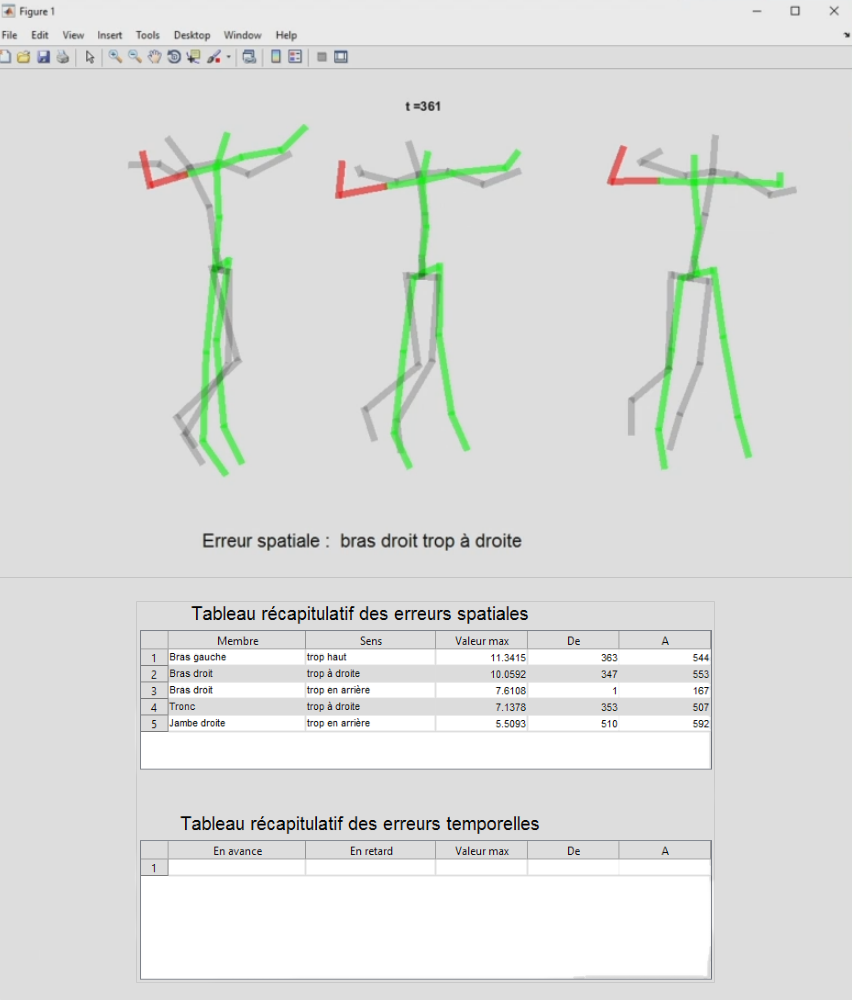
\includegraphics[width=10cm]{pictures/Morel_eiah.png}
    \caption[EIAH pour l'évaluation de gestes sportifs \parencite{Morel2017Mts}]{Le système développé par Morel permet d'afficher les plus grandes erreurs spatiales et temporelles du mouvement de l'apprenant, par rapport à celui de l'expert \parencite{Morel2017Mts}.}
    \label{fig:Morel_eiah}
\end{figure}

Enfin, le système proposé par Le Naour \textit{et al.} a pour but de fournir une aide à l'apprentissage de mouvement en proposant une superposition du modèle de l'apprenant à celui de l'expert, dans un environnement virtuel \parencite{LeNaour2019S3V} (Fig. \ref{fig:LeNaour_eiah}). Les mouvements sont capturés à l'aide d'un système de marqueurs réfléchissants et caméras infrarouges. L'expérimentation présentée dans ces travaux porte sur le lancer au football américain. En premier lieu, une démonstration est effectuée par un expert, et des conseils sont donnés par ce dernier sur les caractéristiques propres à un bon geste (\textit{e.g.} position et rotation des articulations impliquées dans le mouvement, prise de la balle, \textit{etc.}). Après dix lancers d'entraînement, les participants devaient effectuer cinquante lancers, tout en suivant le plus possible le mouvement de l'expert. Plusieurs groupes ont été formés : un groupe sans aucun retour sur la performance, un groupe où le mouvement de l'expert était montré après chaque lancer, un autre où le mouvement de l'expert était montré au participant pendant leur mouvement, suivit de la visualisation de la superposition du mouvement du participant à celui de l'expert, un autre groupe où le mouvement de l'expert était superposé à celui du participant pendant le geste et où le geste de l'expert était visualisé après le lancer, et un dernier où le modèle expert superposé à celui de l'apprenant était visualisé pendant et après le geste. Ont été relevés l'écart-type du calcul de la DTW entre le mouvement de l'apprenant et de l'expert, et la distance par rapport au centre de la cible (le résultat du mouvement). Les résultats montrent que les groupes ayant reçu les retours sous forme de superposition des modèles expert et apprenant ont montrés une amélioration de leur geste. Il est intéressant de noter que l'amélioration du geste n'améliore pas systématiquement la distance par rapport au centre de la cible, et inversement. Ainsi, lors de l'analyse du résultat d'une telle expérimentation, il faut être en mesure de positionner l'objectif final de l'apprentissage : amélioration du geste ou du résultat du geste.

\begin{figure}[h]
    \centering
    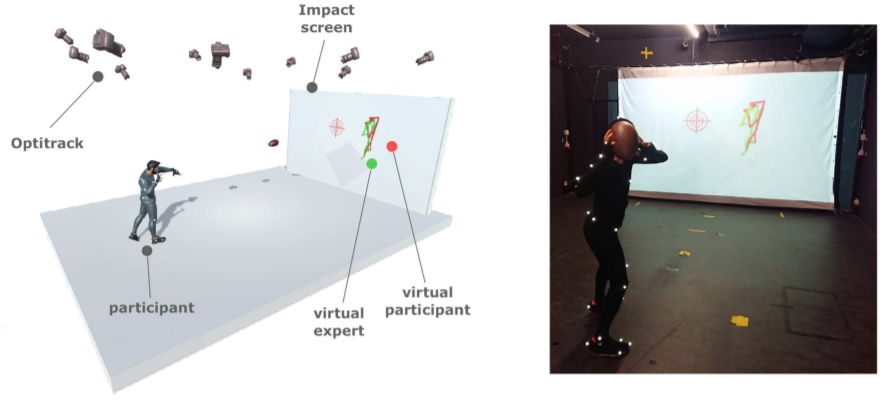
\includegraphics[width=10cm]{pictures/LeNaour_eiah.png}
    \caption[EVAH superposant les gestes de l'apprenant à ceux de l'expert \parencite{LeNaour2019S3V}]{Le système développé par LeNaour \textit{et al.} propose une superposition en temps réel des mouvements de l'apprenant et de l'expert dans un environnement virtuel \parencite{LeNaour2019S3V}.}
    \label{fig:LeNaour_eiah}
\end{figure}

% Probably: Tai-chi sci-hub.tw/10.1109/VR.2017.7892299 \parencite{He2017Iac}

\subsection{Tableau de synthèse}
Tous ces systèmes ont pour point commun d'aider à l'apprentissage de geste, que ce soit en proposant une aide à la décision à l'enseignant, en intégrant les connaissances expertes à un système permettant de s'affranchir de la présence de l'expert, en proposant une évaluation du geste en fonction de critères pré-définis, ou en analysant automatiquement les différences entre les gestes, avec un \textit{a priori} ou non.

Les systèmes où la connaissance experte est intégrée dès la conception permettent de focaliser la conception de l'EIAH sur un problème précis, et ainsi de l'adapter du mieux possible au geste cible (données relevées et utilisées, environnement d'apprentissage du geste, retours à faire à l'apprenant, etc.) \parencite{Baldominos2015AAt, Alankus2010TCG, Gameiro2014KST, BMT_2015, LeNaour2019S3V}. Dans ces cas, il est possible de faciliter l'apprentissage du geste, mais également de proposer des évaluations sous forme de score pertinent dans le contexte applicatif choisi ou de retours donnés par l'expert après visualisation des indicateurs de la performance. Cependant, comme le montre le tableau \ref{tab:eiah_tab}, ces systèmes ne sont pas réutilisables dans d'autres contexte sans nécessiter un processus de réingénierie conséquent : il faut ainsi re-formaliser et réintégrer une autre connaissance experte dans une nouvelle phase de conception, possiblement ré-adapter le système au nouvel environnement dans lequel le geste est réalisé, acquérir de nouvelles données puis les intégrer au processus de traitement, et enfin ré-adapter les retours donnés en fonction des objectifs d'apprentissage.

L'utilisation d'algorithmes d'apprentissage automatique est une méthode qui permet de séparer les gestes de l'apprenant de ceux de l'expert de manière automatique selon des caractéristiques prédéfinies \parencite{Ng2008}. En outre, elle permet également d'observer dans quelle mesure les caractéristiques déterminées au préalable du geste observé varient entre ces mouvements \parencite{BMT_2015}. Ces méthodes nécessitent de disposer d'une base de données d'apprentissage conséquente (\textit{i.e.} de l'ordre du millier de données de mouvement) afin d'être capable de construire une bonne fonction de séparation. En pratique, il est fastidieux de devoir constituer un corpus de données annotées spécifique à un type de mouvement, bien que des bases de données existent (e.g. \textit{Graphics Lab Motion Capture Database} \parencite{CMUDatabase}, \textit{Motion Capture Database HDM05} \parencite{HDM05Database}, \textit{etc.}). Cependant, ces bases sont rarement spécialisées sur une tâche précise, et des variations et spécificités peuvent exister sur le geste à apprendre pour une même tâche et un même enseignant. De plus, l'utilisation d'algorithmes d'apprentissage supervisé suppose d'avoir la connaissance des différentes classes en sortie de l'algorithme, ce qui limite les types de restitution par rapport aux connaissances d'un expert humain, comme montré dans le tableau \ref{tab:eiah_tab}. Bien que l'expert soit en mesure de proposer des caractéristiques, il est possible que les variations de ces caractéristiques puissent mener à la formation de groupes possédant une sémantique plus fine que « réussi / raté » par exemple, permettant de proposer une séparation prenant en compte plusieurs niveaux de réussite du geste, ou menant à la découverte de caractéristiques spécifiques à un type de difficulté ou d'apprenant.

Les systèmes où la découverte des différences significatives entre des groupes de gestes se fait de manière totalement automatique s'affranchissent de l'intégration de la connaissance experte à l'aide du vocabulaire métier, où l'intègrent sous la forme de descripteurs cinématiques, géométriques ou biomécaniques  \parencite{Makio2007DoS} \parencite{Pirsiavash2014AQA}. De nouveaux critères de séparation des gestes acceptables ou non peuvent être découverts. Ils manquent cependant de sémantique dans leur retour : ainsi, il n'est pas possible d'identifier par exemple des groupes ou ensembles de gestes acceptables et non acceptables typiques afin d'étudier les caractéristiques des meilleures stratégies et des erreurs les plus fréquentes. De plus, il peut être difficile de fournir des retours pertinents à des personnes ne possédant pas des compétences poussées en physique, mécanique, \textit{etc.}, car l'interprétation de données cinématiques, géométriques, \textit{etc.} exige d'avoir ces connaissances. Ainsi, les conseils apportés par un tel système doivent non seulement être pertinent dans le contexte applicatif retenu, mais également compréhensibles et utilisables par des personnes sans connaissances scientifiques avancées, ce qui n'est pas toujours réalisable.


\pagebreak
\begin{landscape}
\begin{table}[]
\resizebox{\linewidth}{!}{\begin{tabular}{|l|l|l|l|l|l|l|l|l|l|}
\hline
\multicolumn{1}{|c|}{Auteurs} & \multicolumn{1}{c|}{Domaine} & \multicolumn{1}{c|}{Objectif visé} & \multicolumn{1}{c|}{\makecell[l]{Acquisition\\des données}} & Modélisation des connaissances & \multicolumn{1}{c|}{Analyse} & \multicolumn{1}{c|}{Acteur de la restitution} & \multicolumn{1}{c|}{Information restituée} & \multicolumn{1}{c|}{\makecell[l]{Visualisation du geste\\ou de la restitution}} & \multicolumn{1}{c|}{Généricité} \\ \hline

Yoshinaga et Soga & \makecell[l]{Sport\\Archerie Japonaise} & \makecell[l]{Amélioration du geste\\par rapport aux\\modèles experts} & \makecell[l]{Caméra RGB-D\\(Kinect)} & \makecell[l]{Corpus de squelettes 3D\\ d'experts (enregistrement ad-hoc)} & \makecell[l]{Empirique : analyse visuelle de \\l'expert du squelette 3D de\\l'apprenant effectuant le\\mouvement} & Expert & \makecell[l]{Différences de positions entre les\\mouvements de l'expert et l'apprenant} & \makecell[l]{Superposition de l'apprenant\\et des modèles de coachs} & \makecell[l]{Générique, nécessite de réintégrer\\des modèles experts dans le système} \\ \hline

Kora et al. & \makecell[l]{Sport\\Golf} & Amélioration du swing & \makecell[l]{Caméra RGB-D,\\caméra sur casque\\de réalité virtuelle} & Un modèle d'expert (squelette 3D) & \makecell[l]{Empirique (par l'étudiant) :\\ visualisation des différences\\ entre le modèle expert et son geste} & Aucune restitution & Aucune information restituée & \makecell[l]{Superposition de l'apprenant\\et du modèle expert\\en temps réel} & \makecell[l]{Dépendance totale du système\\au matériel et au domaine applicatif} \\ \hline

Yamaoka et al. & \makecell[l]{Sport\\Lancer de disque} & \makecell[l]{Position des articulations\\lors du lancer} & \makecell[l]{Caméra RGB-D\\(Kinect)} & \makecell[l]{Positon relative des articulations\\entre elles dans les différentes étapes\\du mouvement (défini par un expert)} & \makecell[l]{Automatique : comparaison de\\valeurs à des seuils} & système (textuel) & Positions des membres à corriger & \makecell[l]{Retours générés automatiquement\\à partir de l'analyse} & \makecell[l]{Nécessite de re-formaliser la connaissance experte\\au sein du système (re-conception)} \\ \hline

Ng & \makecell[l]{Musique\\Violon} & \makecell[l]{Détermination du\\style de jeu} & \makecell[l]{Capteurs\\réfléchissants\\(sur l'archet\\et le violon)} & \makecell[l]{Représentation symbolique du son\\(système SMR), descripteurs du\\mouvement (amplitude, vitesse, durée)} & \makecell[l]{Automatique (clustering sur les\\descripteurs extraits)} & \makecell[l]{Enseignant et système\\(visualisation de la\\similitude des\\mouvements entre\\eux)} & \makecell[l]{Mode de jeu, durée, position de l'archet\\ et de l'instrument, vitesse de jeu,\\amplitude du mouvement} & \makecell[l]{Visualisation 3D du mouvement du\\violon et de l'archet, regroupement\\ des mouvements en fonction de\\leurs caractéristiques communes} & \makecell[l]{Dépendance totale du système au matériel\\et au domaine applicatif} \\ \hline

Choi et al. & \makecell[l]{Médical\\Insertion de\\sonde nasogastrique} & \makecell[l]{Apprentissage de la\\procédure d'insertion} & Bras haptique & \makecell[l]{Modèle 3D  de patient vérifiant les\\collisions frictions, etc.\\Procédure complète et étapes clés\\modélisées sous la forme\\d'un arbre de décision} & \makecell[l]{Empirique par l'expert (à partir\\de métriques : durée, min et max\\ de force appliquées, nombre d'insertion\\et nombre de deformations du tube)} & \makecell[l]{Expert (retours\\empiriques) et\\le système\\(retours visuels et haptiques)} & \makecell[l]{Visualisation de la position de la sonde\\dans le modèle 3D, retour de force de\\l'instrument, durée, min et max de\\force appliquées, nombre d'insertion et\\nombre de déformations du tube} & \makecell[l]{Visualisation 3D en temps réel de\\la position de la sonde dans un\\modèle 3D d'humain} & \makecell[l]{Dépendance totale du système au matériel et\\au domaine applicatif} \\ \hline

Baldominos et al. & \makecell[l]{Médical\\Réadaptation\\physique} & Rééducation des patients & \makecell[l]{Caméra RGB-D\\(Intellisense)\\et casque de\\réalité virtuelle\\(Oculus Rift)} & \makecell[l]{Position du patient comparée à des\\références fournies par les médecins\\pour les parties du corps concernées} & Empirique : par l'expert médical & Expert médical & Rééducation suffisante ou non & \makecell[l]{Environnement de réalité virtuelle\\dans lequel le patient\\effectue les gestes désirés} & \makecell[l]{Nécessite de re-formaliser la connaissance experte\\au sein du système (re-conception), re-développemen\\de scène virtuelle, dépendance du système\\au matériel utilisé} \\ \hline

Toussaint et al. & \makecell[l]{Médical\\Chirurgie\\orthopédique\\percutanée} & \makecell[l]{Apprentissage de la\\manipulation de l'objet\\pendant la procédure} & \makecell[l]{Bras haptique\\et occulomètre} & \makecell[l]{Séquences d'actions à effectuer par\\ l'apprenant au cours de l'opération} & \makecell[l]{Automatique : analyse de l'ordre des\\séquences d'action} & Système & \makecell[l]{Propose de revoir une partie du cours,\\consulter un cas clinique ou résoudre\\un autre problème sur le simulateur} & \makecell[l]{Visualisation en temps réel de la\\ manipulation de l'objet} & \makecell[l]{Nécessite de re-formaliser la connaissance experte\\au sein du système, dépendance du système\\au matériel utilisé} \\ \hline

He et al. & \makecell[l]{Sport\\Chinese Taichi} & Apprentissage du Taichi & \makecell[l]{Caméra RGB-D\\(Kinect)} & Squelette 3D de référence pour le geste & \makecell[l]{Automatique : comparaison avec modèle\\expert au niveau de la position\\spatio-temporelle selon 3 métriques} & Système & \makecell[l]{Score prenant en compte les 3\\métriques calculées sur le mouvement\\de l'apprenant par rapport au\\mouvement de l'expert} & \makecell[l]{Environnement de réalité virtuelle\\et CAVE} & \makecell[l]{Nécessite de re-formaliser la connaissance experte\\au sein du système (re-conception)} \\ \hline

Chan et al. & Danse & Apprentissage de la danse & \makecell[l]{Caméra infrarouge\\+ marqueurs} & \makecell[l]{Un modèle d'expert (avatar reproduit\\à l'aide du squelette 3D)} & \makecell[l]{Automatique : comparaison de la position\\ des articulations entre l'apprenant et le\\modèle expert} & Système & \makecell[l]{Visualisation du mouvement de\\ l'apprenant et de celui de l'expert,\\coloration des parties du corps non\\synchronisées avec celles de l'expert} & \makecell[l]{Environnement 3D (OpenGL)\\montrant le squelette de\\l'apprenant et le modèle de\\l'expert en train de réaliser\\ les mouvements de danse} & \makecell[l]{Générique par rapport au domaine applicatif,\\nécessite de réintégrer des modèles experts\\dans le système} \\ \hline

Morel (thèse) & Sport & Amélioration du geste sportif & \makecell[l]{Caméra infrarouge\\+ marqueurs} & Un modèle d'expert (squelette 3D) & \makecell[l]{Automatique : décalage spatial et temporel\\à l'aide de la SDTW} & Système & \makecell[l]{Visuelle et textuelle (affichage des 5\\erreurs les plus significatives,\\ainsi que le temps auquel elles\\apparaissent)} & \makecell[l]{Superposition du mouvement\\de l'apprenant par-dessus\\celui de l'expert, mise en évidence\\des erreurs les plus\\ significatives} & \makecell[l]{Nécessite de re-formaliser la connaissance experte\\au sein du système (re-conception)} \\ \hline

Gaimero et al. & Langue des signes & \makecell[l]{Amélioration du signage\\de l'apprenant} & \makecell[l]{Caméra RGB-D\\(Kinect)} & \makecell[l]{Images des signes fait par un ou\\des expert(s)} & \makecell[l]{Automatique : masquage des données de\\l'apprenant par rapport au bon signe\\présent dans la base de données} & Système & \makecell[l]{Réussite ou non du geste\\(restitution binaire)} & \makecell[l]{Affichage de l'image du geste\\capturé} & \makecell[l]{Nécessite de re-formaliser la connaissance experte\\au sein du système (re-conception)} \\ \hline

Xu et al. & \makecell[l]{Apprentissage\\de gestes\\(pas de contexte\\particulier)} & \makecell[l]{Apprentissage de\\gestes spécifiques} & Caméra RGB-D & Corpus de mouvements unitaires & Automatique : modèle de Markov caché & Système & \makecell[l]{Proposition d'exercices adaptés\\au renforcement de l'apprentissage\\des gestes non-maitrisés} & \makecell[l]{Sur le système, par une\\visualisation du geste correct à\\effectuer et des erreurs} & \makecell[l]{Générique par rapport au domaine applicatif, nécessite\\ de réintégrer des modèles experts dans le système} \\ \hline

Maes et al. & Danse & Apprentissage de la danse & \makecell[l]{Caméra infrarouge\\+ marqueurs} & \makecell[l]{Descripteurs du mouvement\\(déplacement du centre du corps\\par rapport au tempo, rotation du corps\\autour de l'axe vertical)} & \makecell[l]{Automatique : calcul de corrélation\\entre les descripteur du mouvement\\de l'apprenant et de l'expert} & Système & \makecell[l]{Score final, correspondant à la\\similitude entre le geste de l'apprenant\\et celui de l'expert} & Affichage du score & Dépendance totale du système au domaine applicatif \\ \hline

Makio et al. & Sport - générique & \makecell[l]{Séparation des gestes\\expert / apprenant} & Non précisé & Descripteurs du mouvement & Automatique & Système & \makecell[l]{Différence au niveau des\\descripteurs du mouvement calculés} & \makecell[l]{Affichage graphique de la\\différence entre les données\\de l'apprenant et de l'expert} & \makecell[l]{Générique par rapport au domaine applicatif, nécessite\\de réintégrer des modèles experts dans le système} \\ \hline

Le Naour et al. & \makecell[l]{Sport\\lancer au football\\américain} & Amélioration du geste sportif & \makecell[l]{Caméra infrarouge\\+ marqueurs} & \makecell[l]{Descripteurs du mouvement\\et résultat du lancer} & Automatique & Système & \makecell[l]{Différence visuelle entre le mouvement\\de l'apprenant et de l'expert} & \makecell[l]{Visualisation du mouvement\\de l'apprenant superposé\\ou non à celui de l'expert\\(en fonction du groupe)} & \makecell[l]{Nécessite de re-formaliser la connaissance experte\\au sein du système (re-conception)} \\ \hline

\end{tabular}}
\caption{Tableau résumant les principales caractéristiques des EIAH vu dans le chapitre.}
\label{tab:eiah_tab}
\end{table}
\end{landscape}
\pagebreak

%\begin{landscape}
%\begin{table}[]
%\resizebox{\linewidth}{!}{\begin{tabular}{m{2cm}m{2cm}m{2cm}m{3cm}m{3cm}m{2cm}m{7cm}m{7cm}m{7cm}}
%
%Nom (Auteur ?) & Objectif & Domaine & Type de données & Matériel de capture                                                          & Données nécessaire & Visualisation & Analyse & {Retours à l'apprenant}                                                                                                    \\ \toprule
%\parencite{Yoshinaga2015Doa} & Archerie japonaise & Sport & Squelette 3D & Caméra RGB-D (Kinect) & Plusieurs captures d'experts & Superposition de l'apprenant modèles de coachs & Empirique & Par un expert \\\arrayrulecolor{gray}\hline
%\parencite{Kora20151559} & Golf & Sport & Squelette 3D & Caméra RGB-D, caméra sur casque de réalité virtuelle & Un expert & Superposition de l'apprenant et du modèle expert en temps réel & Aucune & Aucun \\\arrayrulecolor{gray}\hline
%\parencite{Yamaoka2013FoF} & Lancer de disque & Sport & Squelette 3D & Caméra RGB-D (Kinect) &  &  & Automatique (positon relative des articulations entre elles dans les différentes étapes du mouvement) & Retours générés automatiquement à partir de l'analyse \\\arrayrulecolor{gray}\hline
%\parencite{Ng2008} & Violon & Musique & Données 3D des positions du violon et de l'archet & Capteurs réfléchissants (sur l'archet et le violon) & Une ou plusieurs & Visualisation 3D du mouvement du violon et de l'archet & Analyse du son, détection automatique du style de jeu à l'aide de clustering &  \\\arrayrulecolor{gray}\hline
%\parencite{Choi2015103} & Insertion de sonde nasogastrique & Médical & Position de l'objet (sonde nasogastrique) & Bras haptique & Une & Visualisation 3D en temps réel de la position de la sonde dans un modèle 3D d'humain & Aucune & Retour de force si la sonde bute contre une paroi du modèle 3D \\\arrayrulecolor{gray}\hline
%\parencite{Baldominos2015AAt} & Réadaptation physique & Médical & Squelette 3D & Caméra RGB-D (Intellisense) et casque de réalité virtuelle (Oculus Rift DK2) & Une & Environnement de réalité virtuelle dans lequel le patient effectue les gestes désirés & Analyse par l'expert médical & Retours empiriques par l'expert médical \\\arrayrulecolor{gray}\hline
%\parencite{BMT_2015} & Chirurgie orthopédique percutanée & Médical & Position de l'objet (trocard) & Bras haptique & Une & EIAH proposant une visualisation en temps réel de la manipulation de l'objet & Automatique (par le système) & Propose de revoir une partie du cours, consulter un cas clinique ou résoudre un autre problème sur le simulateur \\\arrayrulecolor{gray}\hline\
%\parencite{He2017Iac} & Chinese Taichi & Sport & Squelette 3D & Caméra RGB-D (Kinect) & Plusieurs captures d'experts & Environnement de réalité virtuelle et CAVE & Automatique (comparaison avec modèle expert au niveau de la position spatio-temporelle selon 3 métriques) & Score prenant en compte les 3 métriques calculées sur le mouvement de l'apprenant par rapport au mouvement de l'expert \\\arrayrulecolor{gray}\hline
%\parencite{Chan2011} & Danse & Danse & Squelette 3D & Caméra infrarouge + marqueurs & Au moins un expert & Environnement 3D (OpenGL) montrant le squelette de l'apprenant et le modèle de l'expert en train de réaliser les mouvements de danse & Automatique : comparaison de la position des articulations entre l'apprenant et le modèle exper) & Visualisation du mouvement de l'apprenant et de celui de l'expert, coloration des parties du corps non synchronisées avec celles de l'expert\\\arrayrulecolor{gray}\hline
%\parencite{Maes2012DtM} & Danse & Danse & Squelette 3D & Caméras infrarouge & Un modèle expert & Environnement 3D montrant le geste à reproduire, les gestes à réaliser et la superposition de l'apprenant et de l'expert & Automatique : score calculé par le système et empirique : évaluation de l'enregistrement vidéo de la danse par un expert & Score de performance globale donné par le système et (facultatif) évaluation qualitative de l'expert\\
%\bottomrule
%\end{tabular}}
%\caption{Regroupement d'EIAH utilisant différentes modalités pour l'apprentissage du geste.}
%\label{EIAH_table}
%\end{table}
%\end{landscape}

\section{Discussion}
L'apprentissage du geste peut prendre place dans de nombreux contextes. Dans ce chapitre, nous avons vu les différents matériels et EIAHs actuellement utilisés pour l'apprentissage du geste à l'aide d'un environnement informatique. Bien que ces systèmes présentent de nombreuses différences tant au niveau du matériel, que des données utilisées, des retours fait à l'apprenant, des méthodes d'intégration des besoins d'observation et des connaissances de l'expert et de la place de ce dernier dans l'usage, ils ont pour point commun de mettre à la disposition des enseignants et des apprenants un ensemble d'outils permettant de faciliter l'apprentissage, l'analyse ou l'évaluation des gestes. Ces systèmes proposent généralement une analyse du geste, sous une ou plusieurs formes : sous la forme de comparaison visuelle entre les données de l'expert et celles de l'apprenant, en proposant une évaluation sous forme de score, en permettant de visualiser le parcours de l'apprenant dans le cas de multiples gestes qui se suivent, \textit{etc.} L'intégration de l'analyse automatique permet de proposer une aide à l'évaluation, voire de remplacer l'expert dans cette tâche. Bien que l'apprentissage supervisé soit utilisé pour l'analyse de gestes, afin de séparer automatiquement les gestes en fonction de leur sémantique ou de leur degré de réussite, peu de travaux explorent l'utilisation d'algorithmes d'apprentissage non-supervisé. Cela peut s'expliquer par le manque de sémantique associée aux groupes obtenus en sortie. Il est cependant possible d'utiliser un petit nombre de données étiquetées, dans le contexte de l'apprentissage semi-supervisé, afin d'être en mesure de donner un sens aux groupes ainsi obtenus.

Ce chapitre a mis en relief le manque de systèmes assistant l'enseignant qui soient réutilisables dans plusieurs contextes sans une réingénierie conséquente, malgré la variété existante d'EIAH dédiés à l'apprentissage du geste. Une des hypothèses de ce travail de thèse est qu'il est possible de proposer un EIAH réutilisable dans d'autres contextes avec un coût de réingénierie minimisé, accompagnant l'expert dans sa tâche d'enseignement des gestes, en combinant plusieurs des techniques utilisées au sein des systèmes déjà présentés. L'intégration de la connaissance experte en amont de la séance d'apprentissage, puis l'utilisation d'algorithmes d'apprentissage semi-supervisés permettraient de proposer une aide à la décision, en fonction de caractéristiques observées à partir des captures des gestes de l'apprenant. L'avantage d'un tel système serait de permettre à l'enseignant d'analyser toutes les facettes voulues du mouvement sur un même geste, ce qui n'est pas toujours aisé ou possible dans le cadre de mouvements faisant appel à plusieurs parties du corps en même temps (par exemple, l'analyse du jeu d'un étudiant à la guitare).

Que le processus d'analyse soit automatique ou non, il peut être dur d'inférer des informations quant à la bonne réussite du geste ou non à partir de données de mouvement seules. Les EIAH présentés dans cette partie n'utilisent parfois que les données de mouvements capturés. Ces systèmes se basent sur une comparaison du mouvement à une référence, qui peut être l'expert, ou simplement une comparaison des paramètres clés du mouvement avec ceux de référence. Il est ainsi possible ainsi de visualiser les moments de décalages (autant temporels que spatiaux) entre le mouvement de l'apprenant et celui du mouvement attendu. Ces retours donnés à l'apprenant sont cependant souvent " bas-niveau ", c'est-à-dire qu'ils ne sont donnés qu'en terme de valeurs cinématiques, dynamiques, géométriques et nécessitent des connaissances scientifiques afin d'être interprétable par un apprenant. L'adjonction de l'analyse de l'expert n'est pas systématiquement possible, car certains de ces systèmes sont conçus pour pouvoir être utilisés en autonomie.

Ainsi, il faut être en mesure de fournir une analyse fine à l'aide d'indications précises quant aux différentes caractéristiques du geste tout en utilisant le vocabulaire métier du domaine applicatif. Dans ce contexte, il est important d'être capable d'extraire des valeurs plus facilement interprétables à partir de données de mouvements capturés, ou plus spécifiquement adaptées au contexte. Le prochain chapitre présente les différentes informations qu'il est possible d'extraire à partir de mouvements capturés.

